


\begin{figure}
    \centering
    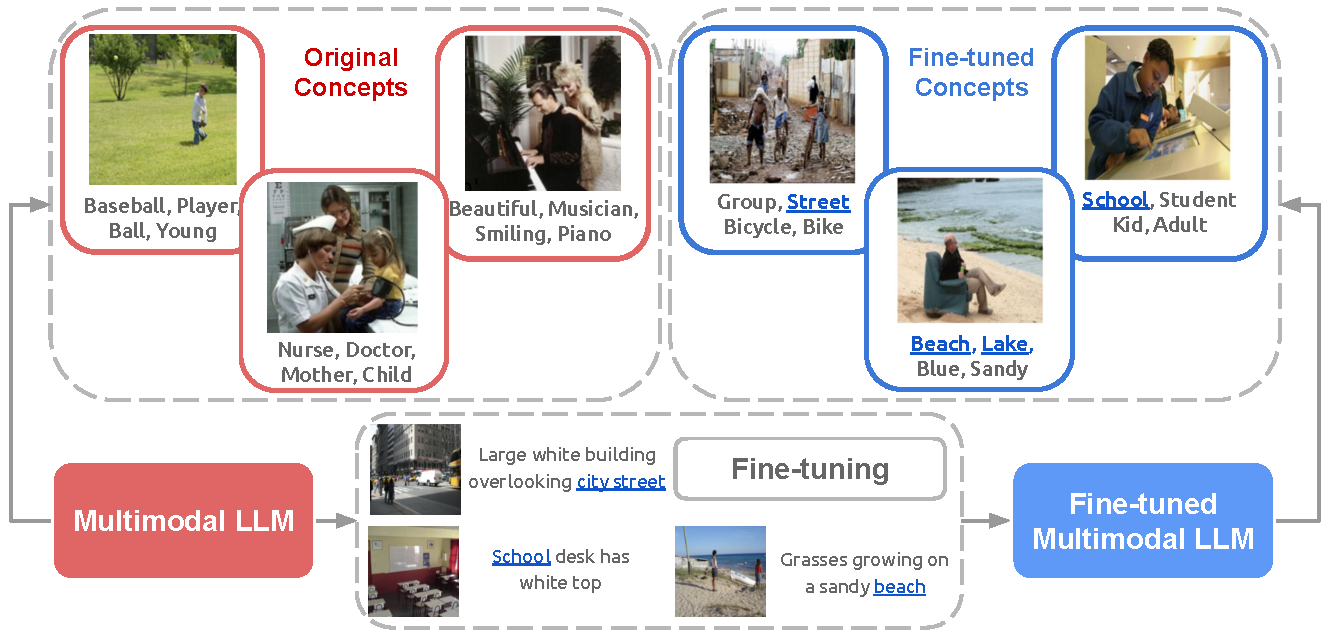
\includegraphics[width=1\linewidth]{Figures/main/mini_teaser.pdf}
    \caption{\textbf{Overview.} We analyse the concepts representations change due to fine-tuning. This has direct implications on steering MLLMs without any extra training.}
\label{fig:mini_teaser}
\end{figure}



With the rapid progress in Large Language Models (LLMs) \cite{brown2020languagegpt3,chowdhery2022palm,openai2023gpt,touvron2023llamav2,jiang2023mistral}, Multimodal LLMs (MLLMs) \cite{driess2023palme,liu2024improvedllava,laurenccon2024mattersidefics2,bai2023qwenvl} have recently demonstrated remarkable capabilities in addressing complex multimodal tasks such as image captioning and visual question-answering. 

MLLMs are typically composed of a visual encoder, an LLM, and an intermediary connector. Following initial unimodal pretraining—and, in many cases, multimodal pretraining on large datasets—these models can be further specialized by training on multimodal datasets \cite{laurenccon2024obelics,flamingo}. Given the high computational cost of training these models, recent research has proposed more efficient approaches, such as creating diverse, high-quality instruction-tuning datasets \cite{liu2024improvedllava} or keeping the LLM frozen and fine-tuning small amount of model parameters, like the connector \cite{shukor2023epalm,manas2023mapl,vallaeys2024improveddepalm,shukor2024skipping}. These approaches take advantage of the impressive ability of frozen LLMs to generalize to multimodal data \cite{shukor2024implicit}. Despite the different efficient tuning methods, training these models still incurs significant cost due to backpropagating the gradient through large models.

While substantial progress has been made in developing high-performing MLLMs, relatively few studies aim to understand them \cite{parekh2024concept,schwettmann2023multimodal,shukor2024beyond,Baldassini_2024_CVPR,zhang2024redundancy,shukor2024implicit}. Existing work typically conducts post-hoc analyses of MLLMs in isolation, overlooking the internal changes during fine-tuning. Research by \cite{shukor2024implicit} addresses this gap to some extent by examining the internal multimodal alignment as it evolves during training. 

In contrast, we focus on exploring how MLLMs update their internal semantic representations when fine-tuned for multimodal tasks (see \Cref{fig:mini_teaser}). Understanding how fine-tuning alters learned concepts—and, consequently, the features encoded by the model—opens the possibility of directly modifying these features to steer model outputs, reducing the need for additional training and its associated costs.


Our approach leverages concept-based explainability to investigate how concept representations evolve from the original model to its fine-tuned version. We find that fine-tuning on a specific task reshapes these concepts, with some adjusting subtly to align with the task, and others emerging or disappearing altogether (see \Cref{fig:teaser}). Notably, most fine-tuned concepts can be reconstructed from the original model by translating its original concepts along specific shift vectors. Lastly, we explore the implications of this study for steering MLLMs, demonstrating how model responses can be modified without additional training. Our key findings are summarized as follows:

\begin{itemize} 
    \item We show that learned concepts adapt specifically to the fine-tuning task, with some concepts becoming more specialized and others undergoing complete transformation. 
    \item Many of the concepts encoded in the fine-tuned model can be reconstructed from those in the original model using shift vectors in the latent space. 
    \item We apply these findings to steer MLLMs (\emph{e.g.}, LLaVA) outputs, demonstrating the possibility to steer the model’s answers or response style. To the best of our knowledge, this is the first work exploring MLLMs steering.
\end{itemize}














